% ------------------------------------------------------------------------------
% TYPO3 Version 9.3 - What's New - Chapter "Backend User Interface" (German Version)
%
% @author	Michael Schams <schams.net>
% @license	Creative Commons BY-NC-SA 3.0
% @link		http://typo3.org/download/release-notes/whats-new/
% @language	German
% ------------------------------------------------------------------------------
% LTXE-CHAPTER-UID:		07b25346-95b1df21-a6ebe09a-49f53f41
% LTXE-CHAPTER-NAME:	Backend User Interface
% ------------------------------------------------------------------------------

\section{Backend User Interface}
\begin{frame}[fragile]
	\frametitle{Backend User Interface}

	\begin{center}\huge{Kapitel 1:}\end{center}
	\begin{center}\huge{\color{typo3darkgrey}\textbf{Backend User Interface}}\end{center}

\end{frame}

% ------------------------------------------------------------------------------
% LTXE-SLIDE-START
% LTXE-SLIDE-UID:		0e8a90f8-5da86aa6-7e9a32fb-20b0bd01
% LTXE-SLIDE-TITLE:		Search Engine Optimization
% ------------------------------------------------------------------------------

\begin{frame}[fragile]
	\frametitle{Backend User Interface}
	\framesubtitle{Suchmaschinenoptimierung}

	Die Seiteneigenschaften verfügen über einen neuen Tab "SEO", mit dem BE-Benutzer 
	SEO-bezogene Informationen, \href{http://ogp.me/}{Open Graph}-Daten und vieles mehr konfigurieren können.

	\begin{figure}
		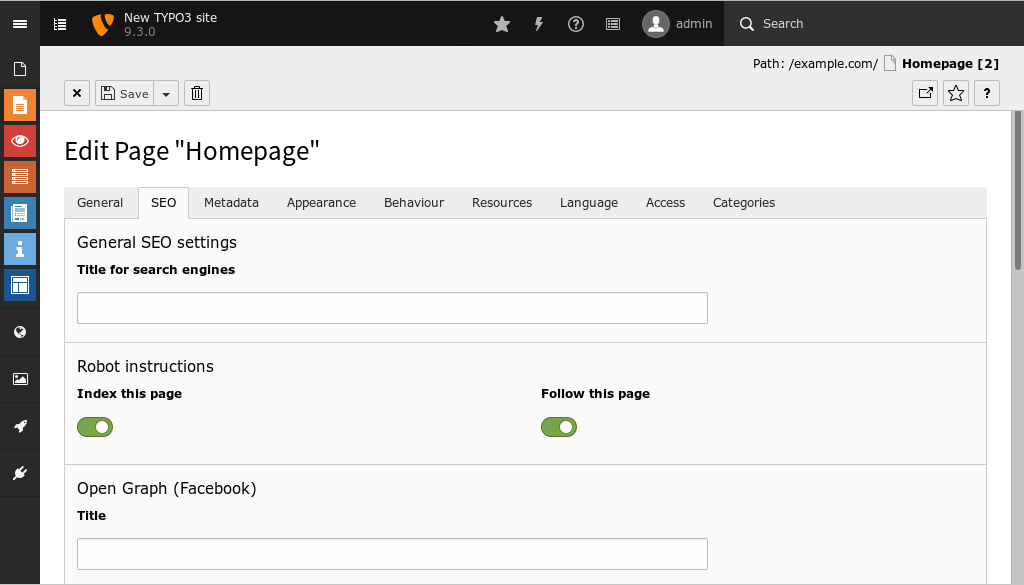
\includegraphics[width=0.70\linewidth]{BackendUserInterface/SearchEngineOptimizationPageProperties.png}
	\end{figure}

\end{frame}

% ------------------------------------------------------------------------------
% LTXE-SLIDE-START
% LTXE-SLIDE-UID:		0e80eecb-f66842d4-e73c50c8-c2bb58a6
% LTXE-SLIDE-TITLE:		Filebrowser Search (Image Meta Data)
% LTXE-SLIDE-REFERENCE:	#71644 - Add metadata to filebrowser search
% ------------------------------------------------------------------------------

\begin{frame}[fragile]
	\frametitle{Backend User Interface}
	\framesubtitle{Filebrowser Suche}

	Wenn die Suchfunktionalität in \textbf{FILE → Filelist} verwendet wird, werden die Metadaten
	der Dateien (z.B. die Felder "Titel", "Beschreibung" and "Alternativer Text") ebenfalls
	durchgesucht.

	\begin{figure}
		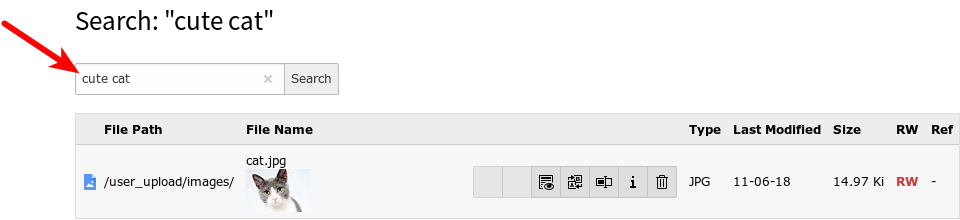
\includegraphics[width=0.90\linewidth]{BackendUserInterface/FilebrowserSearchMetaData.png}
	\end{figure}

\end{frame}

% ------------------------------------------------------------------------------
